%************************************************
\chapter{Kernfaktoren einer sozialen Netzwerkanalyse}\label{ch:kernfaktoren} % $\mathbb{ZNR}$
%************************************************
In komplexen Netzwerken können einige Knoten als wichtiger angesehen werden als andere. In einem sozialen Netzwerken zeichnen sich manche Knoten durch vergleichsweise mehr Verbindungen als andere Knoten aus. Auf das Beispiel \textit{Instagram} bezogen, können solche Knoten Informationen leichter verbreiten, als gewöhnliche Personen, sogenannte Influencer. Daher können diese Knotenpunkte als zentral interpretiert werden. Die Interpretation der Zentralität ist jedoch nicht eindeutig \cite{GOLBECK201325}. Zum Beispiel im Linienverkehr,
gilt eine Linie als zentral, wenn sie von großen Menschenmengen genutzt wird und stärker frequentiert wird
als andere Linien. Die Definition der Zentralität ist also nicht allgemein und hängt von der der Anwendung ab. Da es keine allgemeine Definition von Zentralität gibt, wurden mehrere Maße entwickelt, die jeweils spezifische Konzepte berücksichtigen.
Die Zentralität ist eine Schlüsseleigenschaft komplexer Netzwerke. Sie kann unter anderem das Verhalten dynamischer Prozesse und beispielsweise epidemische Ausbreitung erklären, modellieren und abschätzen, jedoch nicht beschreiben. \cite{SpringerElbert}. Zudem kann die Zentralität Informationen über die Organisation komplexer Systeme, wie unser Gehirn, und unsere Gesellschaft liefern. Es gibt viele Metriken zur Quantifizierung der Knotenzentralität in Netzwerken \cite{francisco}. Nun folgt ein Überblick, über die wichtigsten Zentralitätsmaße und die Hauptmerkmale dieser.

\section{Gradzentralität}
Die Gradzentralität ist die am einfachsten zu berechnende Zentralität. Sie ist definiert durch die Anzahl der Verbindungen, die mit jedem Knoten \textit{direkt} verbunden sind. Mit der Adjazenzmatrix wird der Grad der Zentralität berechnet, indem die Summe der Elemente der betroffenen Zeile $i$ berechnet wird.
Mathematisch formuliert, wird folgende Formel verwendet: 
\begin{equation}
     k_i &= \sum_{j=1}^{N} A_i_j 
\end{equation}

Wobei $A$ die Adjazenzmatrix beschreibt, $N$ die Anzahl an Knoten darstellt und $i$, $j$ die Knoten. \\
Da es sich bei der Gradzentralität um die einfachste Zentralität handelt, wird meist davon ausgegangen, dass Knoten mit vielen Verbindungen, daher mit einer hohen Zentralität, sich im Zentrum eines Netzwerkers befinden. Dies hat jedoch einige Nachteile, denn Knoten mit der höchsten Grad-Zentralität können sich auch am Rand des Netzes befinden, sich daher nicht im Zentrum befinden, was dazu führt, dass die Gradzentralität nicht als lokales Maß betrachtet wird. Zudem sollte hervorgehoben werden, dass bei der Gradzentralität nur ein- beziehungsweise ausgehende Kanten gezählt werden. Die sagt zwar aus, dass ein solcher Knoten, auf das soziale Netzwerk bezogen, eine beliebte oder sehr bekannte Person ist, doch ist keine Aussage über die Macht oder den Einfluss der Person ermöglicht. Als extremes Gegenbeispiel, warum die Gradzentralität nicht immer optimal zur Netzwerkanalyse ist, diene ein Netzwerk mit einer großen, dichten Gruppen von Knoten. Diese machen den größten Teil des Graphen aus, was auch manchmal als Kern des Netzes bezeichnet wird. Jedoch kann (visuell betrachtet) weit außerhalb des Kerns, entlang einer Kette von Knoten mit niedrigem Grad, ein Knoten liegen, der mit einer großen Anzahl von Knoten verbunden ist
verbunden ist. Ein solcher Knoten hätte einen hohen Grad an
Zentralität, obwohl er weit vom Kern des Netzes und den meisten Knoten entfernt ist, in visueller Hinsicht \cite{SpringerElbert}. 
Um solche Faktoren mit berücksichtigen zu können, möchten wir einen weiteren Faktor mit in die Berechnung integrieren, nämlich die Weglänge. Diese spielt eine wichtige Rolle bei der $"$Nähe-Zentralität$"$.  
\section{Nähe-Zentralität}
Als nächstes möchten wir einen weiteren Faktor betrachten, woraus wie eine neue Formel herleiten können, nämlich die Weglänge. Denn die Knotenzentralität kann auch anhand der kürzesten Wege defininiert werden. Der Abstand zwischen zwei Knoten $i$ und $j$ ist gegeben durch die Anzahl der Kanten, welcher sie verbindet. Ein zentraler und daher wichtiger Knoten liegt, bezogen auf den Abstand, nahe an allen anderen Knoten des Netzes. Dieser Gedanke ist im Maß der sogenannten $"$Nähe-Zentralität$"$ oder $"$Closeness-Centrality$"$ enthalten. Diese wird durch den durchschnittlichen Abstand eines jeden Knotens zu allen anderen Knoten definiert. Mathematisch wird die Formel wie folgt beschrieben: 

\begin{equation}
     C_i &= \frac{N}{\sum_{j=1, j \not{=}i}^{N} d_i_j }
\end{equation}

Dabei ist mit $d_i_j$ der kürzeste Weg zwischen $i$ und $j$ gemeint und mit $N$ erneut die Anzahl an Knoten im Netzwerk \cite{SpringerElbert}. Die Nähe-Zentralität ist vor allem dann sehr geeignet, wenn Prozesse über kurze Wege charakterisiert werden wollen. Betrachten wir beispielsweise den hierarchischen Aufbau eines Unternehmens. Dieses kann in einem sternförmigen Graphen dargestellt werden. In der Mitte des Graphen befindet sich der Vorstand, der in engem Kontakt mit den jeweiligen Abteilungsleitern steht. Die Abteilungsleiter sind, neben dem Vorstand, wiederum in sehr nahem Kontakt mit ihren jeweiligen Mitarbeitern ihrer Abteilung. Wenn wir nun ausschließlich anhand der Grad-Zentralität argumentieren würden, wären die Abteilungsleiter die wichtigsten Knoten im Graphen. Jedoch haben diese nicht die niedrigste Nähe-Zentralität, denn der Vorstand hat, da sich dieser Knoten in der Mitte des Graphen befindet, zu allen anderen Knoten entweder einen oder zwei Kanten Abstand. Die einzelnen Abteilungsleiter haben aber im worst-case zu anderen Angestellten aus anderen Abteilungen zwei bis drei Kanten Abstand. Dementsprechend ist es wichtig, auch die Nähe-Zentralität zu betrachten, denn diese ist von hoher Bedeutung. Tatsächlich weisen die meisten komplexen Netze eine geringe durchschnittliche Länge des kürzesten Weges auf. Dies ist dadurch zu begründen, da die typische Entfernung mit dem Logarithmus der Anzahl der Knoten zunimmt. 
Daher liegt das Verhältnis zwischen dem größten und dem kleinsten Abstand
in der Größenordnung $log(N)$, da der minimale Abstand gleich eins ist. In den meisten real existierenden
Netzwerken beträgt dieses Verhältnis etwa sechs oder weniger. Es kann also mehrere Knoten mit der gleichen
Zentralität haben, obwohl sie bei der Informationsverbreitung unterschiedliche Rollen spielen können. Daher ist die Nähe-Zentralität besser geeignet für räumliche Netze, bei denen die Abstände zwischen den Knoten größer ist als in zufälligen Netzen mit der gleichen Anzahl von
Knoten und Verbindungen \cite{SpringerElbert}.

\section{Betweeness-Zentralität}
Die Bewteenesss-Zentraität misst, wie wichtig ein Knoten für die kürzesten Pfade durch das Netz ist. Um diese Zentralität für einen Knoten $N$ zu berechnen, wird in dieser Methode eine Gruppe Knoten ausgewählt und alle kürzesten Wege zwischen diesen Knoten gefunden. Dann wird der Anteil dieser kürzesten Wege berechnet, die den Knoten $N$ einschließen. Wenn es beispielsweise sieben kürzeste Wege zwischen einem Knotenpaar gibt und fünf davon durch den Knoten N führen, dann wäre der Anteil $5/7=0.714$. Dieser Vorgang wird für jedes Knotenpaar im Netz wiederholt. Anschließend werden die berechneten Bruchteile addiert, wodurch die Betweeness-Zentralität des Knotens $N$ generiert wird. Mathematisch formuliert sieht die Formel dann wie folgt aus: 
\begin{equation}
     B_i &= \sum_{(a-b)}\frac{\eta(a,i,b)}{\eta(a,b)}
\end{equation}
Hierbei bezeichnet $\eta(a,i,b)$ die Anzahl der kürzesten Wege zwischen den Knoten $a$ und $b$ die durch den Knoten $i$ führen. Zudem stellt $\eta(a,b)$ die Gesamtzahl der kürzesten Wege zwischen $a$ und $b$ dar. 
Diese Zentralität, basierend auf dem $"$ random walk$"$-Algorithmus, ist gegeben durch die erwartete Anzahl der Besuche jedes Knotens $i$ während einer zufälligen Schrittfolge durch den Graphen:
\begin{equation}
     B_i &= \sum_{a=b}^{N}\sum_{b=1}^{N}w(a,i,b)
\end{equation}
dabei ist $w(a,i,b)$, wie oben bereits beschrieben für $\eta(a,i,b)$, die Anzahl der kürzesten Wege zwischen den Knoten $a$ und $b$ die durch den Knoten $i$ führen. Die Lösung wird nur angenähert.
Die Betweeness-Zentralität ist eines der am häufigsten verwendeten Zentralitätsmaße. Sie gibt an, wie wichtig ein Knoten für den Informationsfluss von einem Knoten des Netzes zu einem anderen ist. In gerichteten Netzwerken kann Betweenness mehrere Bedeutungen haben \cite{SpringerElbert}. Einem Nutzer mit hoher Betweeness-Zentralität folgen möglicherweise viele andere Nutzer, die jedoch nicht denselben Personen folgen wie der Nutzer selbst. Dies würde darauf hindeuten, dass der Nutzer viele Anhänger oder Follower hat. Es kann aber auch sein, dass der Nutzer weniger Follower hat, diese aber dafür mit vielen Konten verbindet, die ansonsten weit entfernt sind. Dies würde darauf hindeuten, dass der Nutzer ein Anhänger von vielen Personen ist, beziehungsweise vielen Personen folgt. Daher ist es enorm wichtig die Richtung der Kanten eines Knotens zu kennen, um die Bedeutung der Zentralität zu verstehen.


\section{Eigenvektor-Zentralität}
Die Eigenvektor-Zentralität misst die Bedeutung eines Knotens, wobei die Bedeutung seiner Nachbarn berücksichtigt wird. Daher wird sie manchmal verwendet, um den Einfluss eines Knotens im Netzwerk zu messen. Er wird durch eine Matrixberechnung ermittelt, um den so genannten $"Haupteigenvektor"$ anhand der Adjazenzmatrix zu bestimmen. Mathematisch betrachtet ist die Eigenvektor-Zentralität die komplizierteste, der in dieser Arbeit betrachteten Zentralitäten.\\
Wir gehen nun von der Vorstellung aus, dass ein Akteur zentraler ist, wenn er in Beziehung zu Akteuren steht, die selbst zentral sind. Wir können also argumentieren, dass die Zentralität eines Knotens nicht nur von der der Anzahl seiner Nachbarknoten abhängt, sondern auch von deren Zentralitätswert. Beispielsweise definiert Bonacich (1972) die Zentralität $c(v_i)$ eines Knotens $v_i$ als positives Vielfaches der Summe der benachbarten Zentralitäten. Als Formel mathematisch dargestellt sieht dies folgendermaßen aus:
\begin{equation}
     \lambda c(v_i) = \frac{1}{\lambda} \sum_{j=1}^{N}a_{ij}c(v_j) \forall i
\end{equation} oder umgeschrieben:  
\begin{equation}
     c(v_i) = \sum_{j=1}^{N}a_{ij}c(v_j) \forall i
\end{equation}
Hierbei repräsentiert $a_{i,j}$ die Werte der Adjazenzmatrix $A$ und $\lambda$ einen konstanten Faktor. \\
In Matrixschreibweise mit $c = (c(v_1), ...., c(v_n))$ bedeutet dies auch:
\begin{equation}
     Ac = \lambda c
\end{equation}
Diese Art von Gleichung wird durch die Eigenwerte und Eigenvektoren von $A$ gelöst.
Aus der gesamten Menge an verschiedenen Eigenvektoren, scheint nur einer eine geeignete Lösung zu sein. 
Dieser Eigenvektor kann dann direkt als Zentralitätsmaß dienen. Da A die Adjazenzmatrix eines ungerichteten (zusammenhängenden) Graphen ist, ist A nicht negativ und aufgrund des Satzes von Perron-Frobenius, gibt es einen Eigenvektor des maximalen Eigenwerts mit nur nicht negativen, also positiven, Einträgen \cite{brittaRuhnau}.

\section{Cliquen und Brücken}


\section{Ein typisches soziales Netzwerk}
Nachdem nun alle Zentralitäten und deren Berechnungen bekannt sind, ist es an der Zeit ein Musterbeispiel für ein soziales Netzwerk zu betrachten. Google Maps ist beispielsweise ein Netzwerk, bei dem die Knoten die \textit{Orte} und die Kanten die \textit{Straßen} sein können. Das bekannteste Netzwerk ist natürlich Facebook. Bei dieser sozialen Plattform ist die geeignetste Darstellung ein \textit{ungerichteter} Graph. Bei Instagram hingegen, ein \textit{gerichtet} Graph. Denn hier gibt es neben Leuten, denen wir folgen, unsere eigenen Follower \cite{fbInsta}. Die Knoten sind die \textit{Nutzer} und die \textit{Kanten} sind die Verbindungen zwischen ihnen. Beachten Sie, dass sowohl \textit{Knoten} als auch \textit{Kanten} Attribute haben können. Knotenattribute in Facebook können zum Beispiel \textit{Geschlecht}, \textit{Ort}, \textit{Alter} usw. sein, und Kantenattribute können \textit{Datum der letzten Unterhaltung zwischen zwei Knoten}, \textit{Anzahl der Likes}, \textit{Datum der Verbindung} usw. sein \cite{GOT}.
Nun wollen wir uns jedoch auch ein typisches soziales Netzwerk anschauen. Wir müssen uns jedoch stets bewusst sein, dass es sich hierbei um einen Datensatz von einem fiktives Fantasy Drama handelt. Genauer gesagt nehmen wir den Datensatz von Game of Thrones zu Hand und betrachten eine bereits durchgeführte SNA genauer \cite{GOT}:

\begin{figure}[h!]
    \centering
    %\hspace*{-1cm}
    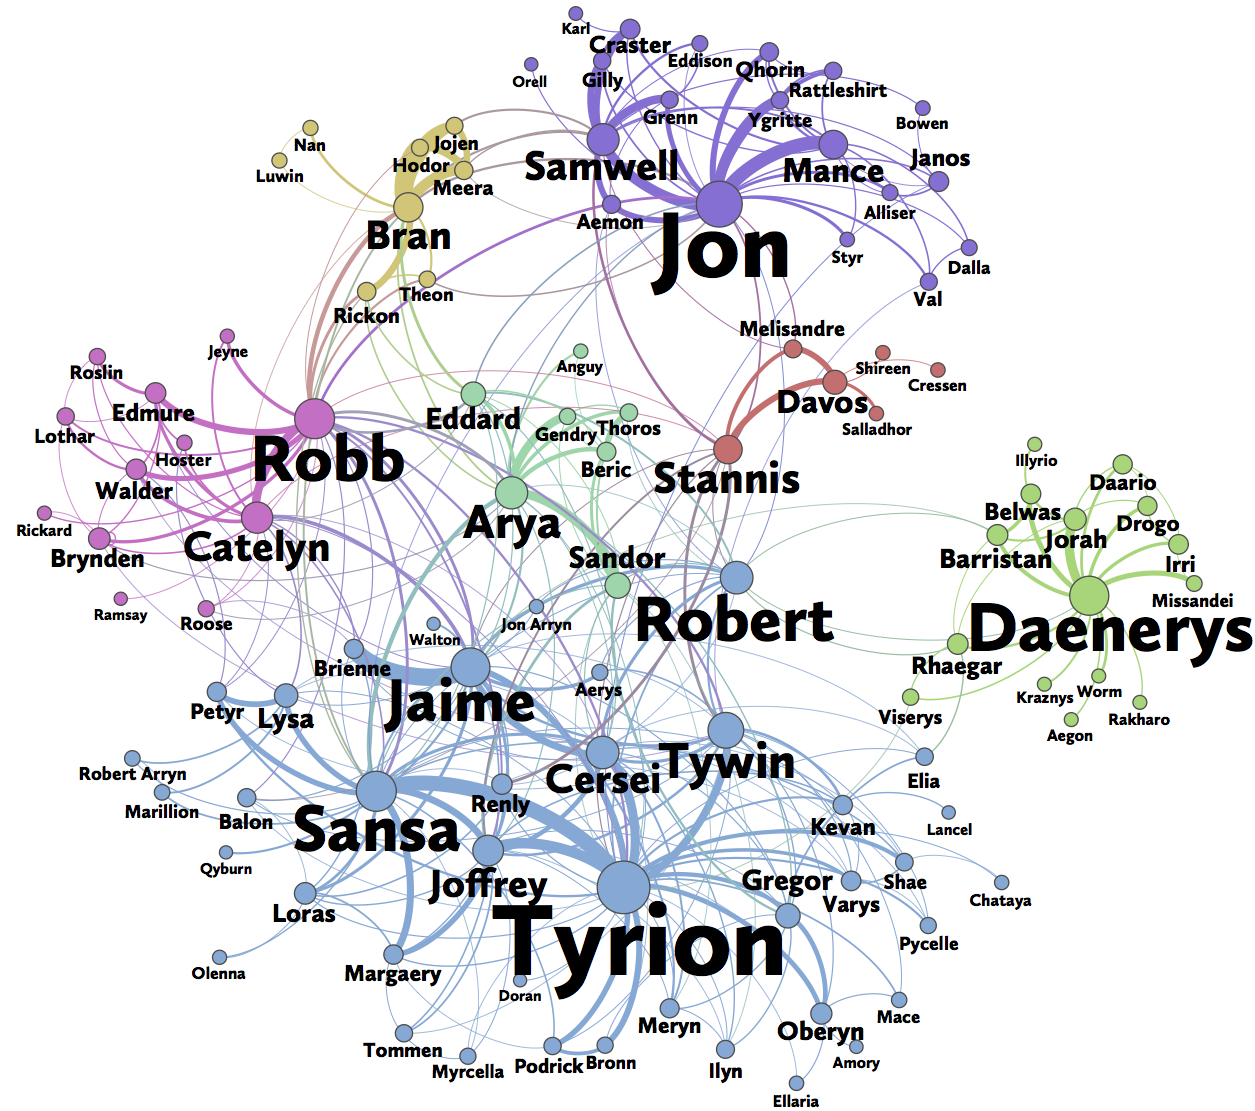
\includegraphics[width=0.75\textwidth]{Graphics/got-network.png}
    \caption{Game of Thrones social Network,\\
    Quelle: https://predictivehacks.com/social-network-analysis-of-game-of-thrones/,\\ Stand: 28.03.2022}
    \label{fig:GameOfThrones}
\end{figure}

Für diesen Plot wurde die $"NetworkX"$ Python-Bibliothek auf $"$Game of Thrones$"$-Daten (GOT) angewendet. Das Netzwerk besteht aus $796$ Knoten und $2823$ Kanten. Insgesamt daher aus $796$ Charakteren aus GOT.\\
In dieser SNA tauchen auch bisher unbekannte Messungen auf, die aber im Interpretations-Teil dieser Arbeit ebenfalls aufgegriffen werden. Beispielsweise beträgt der $"$Durchmesser$"$ des GOT Graphen $9$. Die heißt, wenn die kürzeste Pfadlänge von jedem Knoten zu allen anderen Knoten berechnet ist, ist der Durchmesser die längste aller berechneten Pfadlängen. Die durchschnittlich kürzeste Pfadlänge beträgt $3.41$. Diese werden wir uns aber zu einem späteren Zeitpunkt anschauen. Im Graphen ist gut zu erkennen, welche Knoten eine zentrale Rolle in diesem Graphen spielen. Hierfür wird mit der Knoten-Größe variiert. Große Knoten implizieren, dass es sich um einen wichtigen Knoten für diesen Teilgraphen handelt und kleine, dass es sich um weniger relevante Knoten handelt \cite{GOT}. 
\begin{table}[h!]
\footnotesize
\caption{Werte GOT Graph}
\label{TableGOT}
\begin{tabular}{lccccc}\toprule 
\textbf{Charakter} &\textbf{Grad-Zentr.} & \textbf{Charakter} &\textbf{Nähe-Zentr.}  & \textbf{Charakter} &\textbf{Betweeness-Zentr.} \\
 &\\\midrule
  Tyrion Lannister & 0.1535  & Tyrion Lannister & 0.4763 & Jon Snow& 0.1921   \\
  Jon Snow & 0.1434 & Robert Baratheon & 0.4593 & Tyrion Lannister & 0.1622   \\
  Jaime Lannister & 0.1270  & Eddard Stark& 0.4558& Daenerys Targaryen & 0.1184   \\
  Cersei Lannister & 0.1220 & Cersei Lannister & 0.4545 & Theon Greyjoy & 0.1113   \\
  Stannis Baratheon & 0.1119 & Jaime Lannister & 0.4520 & Stannis Baratheon & 0.1101   \\
       
  \\\bottomrule
 \end{tabular}
 \end{table}
Wenn wir diese in der Abbildung \ref{fig:GameOfThrones} suchen, sehen wir, dass es sich hierbei um die Knoten handelt, die mit den meisten Kanten verbunden sind. Oftmals ist bei den Graphen nicht eindeutig zu erkennen, ob es sich hierbei um Kanten handelt, die zum Knoten führen und sozusagen eine eingehende Kante darstellen, oder diese nur am Knoten vorbei verlaufen. Deshalb ist es wichtig, die Werte aus der Tabelle \ref{TableGOT} zu analysieren. Betrachten wir die Spalten der $"Charakter"$, fällt vor allem auf, dass $"Tyrion -Lannister"$ in allen  Spalten aufgeführt wird. Das heißt, dass dieser Knoten im Graphen sowohl zentral liegen muss, zudem kurze Abstände zu den anderen Knoten nachweisen und über diesen Knoten verlaufen zudem die häufigsten kürzesten Wege. Werfen wir nun einen Blick auf den Graphen \ref{fig:GameOfThrones}, so sehen wir, dass der Knoten, beziehungsweise Charakter, $Tyrion$  sofort auffällt. Er liegt zwar nicht komplett mittig im Graphen aber ist von den meisten Knoten und Kanten umgeben. Da drei der fünf wichtigsten Konten  in der Spalte $Grad-Zentr.$ den gleichen zweiten Namen tragen, liegt die Vermutung nahe, dass es sich hier um Knoten handelt, die auch sehr nah beieinander sein müssten. Beim Betrachten des Graphen bestätigt sich diese Vermutung erneut, denn alle drei Knoten befinden sich im blauen Teilgraphen. Zudem haben Recherchen ergeben, dass es sich bei dem Namen $"Lannister"$ um ein Adelshaus in der US-amerikanischen Fantasy-Fernsehserie $"$Game of Thrones$"$ handelt. Zudem fällt sofort auf, dass drei der fünf Charaktere in der Spalte $Nähe-Zentr.$ bereits die selben sind, wie die wichtigsten Charaktere bezüglich der $Grad-Zentr.$. Wieder bedeutet das, dass diese Charaktere sowohl zentral im Graphen liegen müssen und zudem die kürzesten Wege zu anderen Knoten besitzen. Die Betrachtung von \ref{fig:GameOfThrones} bestätigt dies sofort. Zudem weist der Graph auch einige cliquen auf, die relevanteste und vor allem größte Clique befindet sich im blauen, grünen, ein Knoten im roten und zwei Knoten im pinken Teilgraphen. Jedoch werden wir die Analyse dieses interessanten sozialen Netzwerks nicht weiterführen, sondern uns auf die Analyse des künstlich erstellen sozialen Netzwerks, zu einem späteren Zeitpunkt in dieser Arbeit, fokussieren. Auch der Frage welcher mathematische bzw. stochastische Verteilung die Zentralitäten entsprechen und warum eine solche Untersuchung sinnvoll ist, werden wir zu einem späteren Zeitpunkt nachgehen.


\section{Kurzes Recap}
Nun sind die wichtigsten Eigenschaften der, in dieser Arbeit betrachteten und verwendeten, Zentralitäten bekannt und eingeführt. Manche Zentralitäten wurden oberflächlicher erklärt als andere, was die simple Begründung hat, dass sie weniger relevant für die Untersuchung der sozialen Netzwerke sind. Schließlich haben wir uns gemeinsam ein Beispiel für ein soziales Netzwerk angeschaut und dieses oberflächlich analysiert.

%*****************************************
%*****************************************
%*****************************************
%*****************************************
%*****************************************
